\documentclass{scrartcl} 
\usepackage[utf8]{inputenc} 
\usepackage[OT1]{fontenc} 
\usepackage[dvipsnames]{xcolor}
\usepackage{tikzrput}
\usepackage[object=vectorian]{pgfornament} 

\usetikzlibrary{decorations,decorations.text}



\begin{document}  
\tikzset{pgfornamentstyle/.style={draw = Periwinkle,
                                  fill = SpringGreen}}   
\unitlength=1cm   

\begin{center}   
\begin{picture}(10,10)%
  \color{blue}%
   \put(0,0){\framebox(10,10){%
   \rput[tl](-3,5){\pgfornament[width=6cm]{71}}%
   \rput[bl](-3,-5){\pgfornament[width=6cm,,symmetry=h]{71}}%
   \rput[tl](-5,5){\pgfornament[width=2cm]{63}}%
   \rput[tr](5,5){\pgfornament[width=2cm,,symmetry=v]{63}}%
   \rput[bl](-5,-5){\pgfornament[width=2cm,,symmetry=h]{63}}%
   \rput[br](5,-5){\pgfornament[width=2cm,,symmetry=c]{63}}%
   \rput[bl]{-90}(-5,3){\pgfornament[width=6cm]{46}}%
   \rput[bl]{90}(5,-3){\pgfornament[width=6cm]{46}}%
   \rput(0,0){\Huge \color{MidnightBlue} Ornaments}%
   \rput[t](0,-0.5){\pgfornament[width=5cm]{75}}%
   \rput[b](0,0.5){\pgfornament[width=5cm]{69}}%
   \rput[tr]{-30}(-1,2.5){\pgfornament[width=2cm]{57}}%
   \rput[tl]{30}(1,2.5){\pgfornament[width=2cm,symmetry=v]{57}}}}% 
\end{picture} 
\end{center}
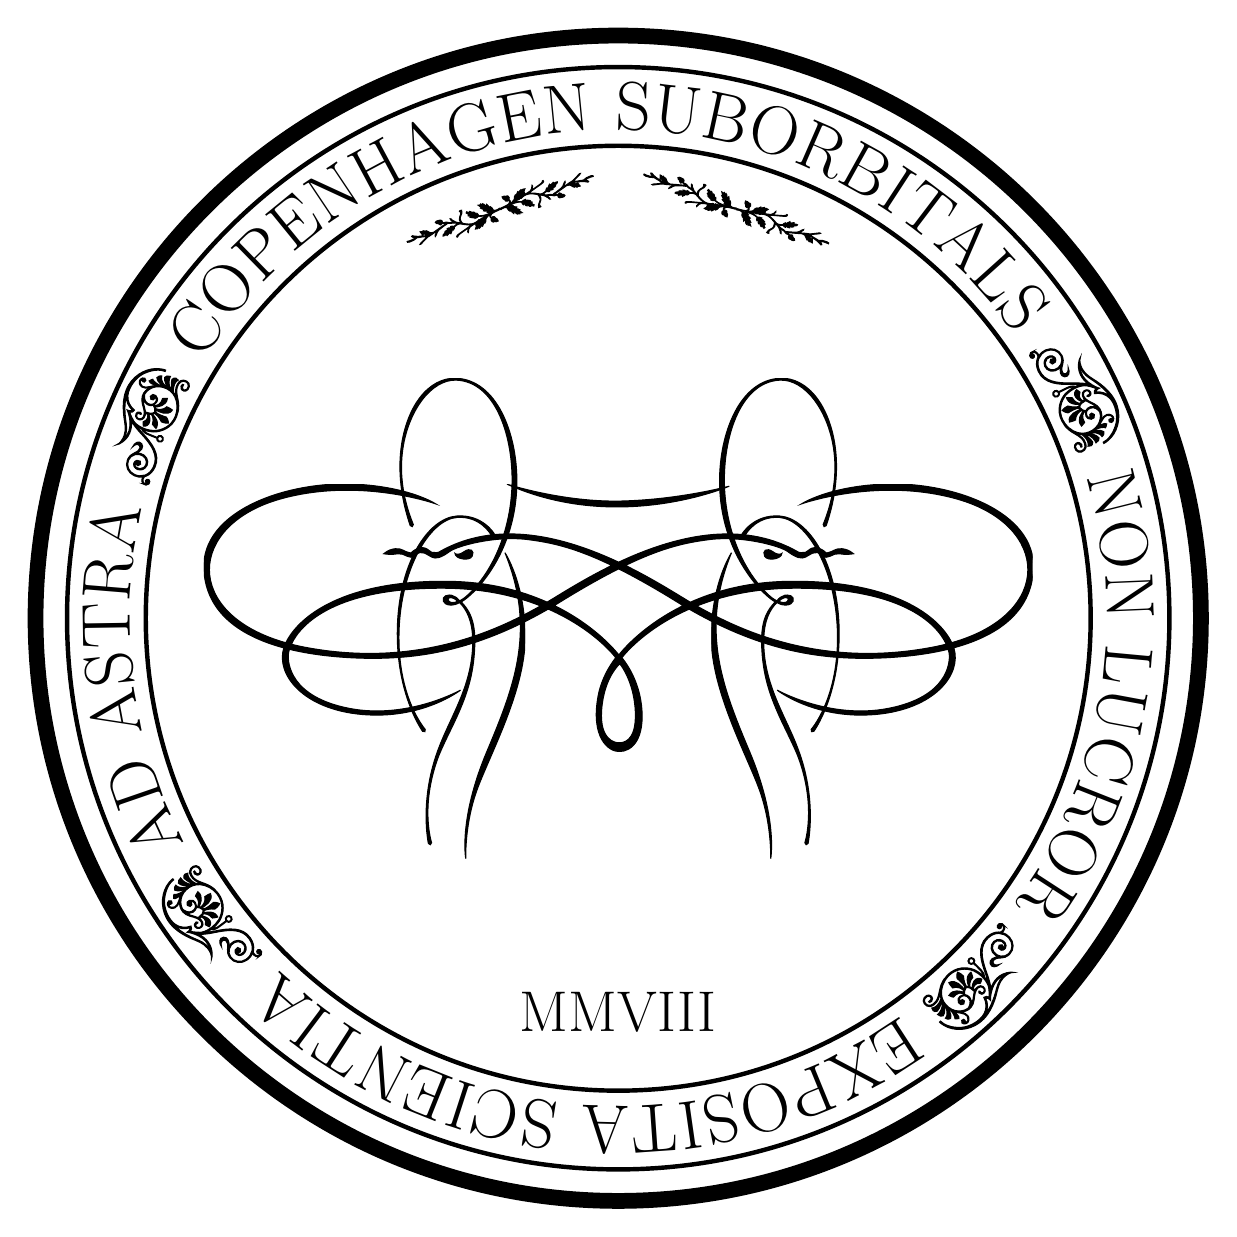
\begin{tikzpicture}

\draw[ultra thick] circle[radius=6cm] circle[radius=7cm]  ;
\draw[line width=2mm] circle[radius=7.4cm]  ;

\path 
    [rotate=210,postaction={decoration={text along path,text format delimiters={|}{|}, text={|\Huge| AD ASTRA {\pgfornament[scale=.4,ydelta=-9pt]{15}} COPENHAGEN SUBORBITALS {\pgfornament[scale=.4,ydelta=-9pt]{15}} NON LUCROR {\pgfornament[scale=.4,ydelta=-9pt]{15}} EXPOSITA SCIENTIA {\pgfornament[scale=.4,ydelta=-9pt]{15}}},
      text align=fit to path,reverse path}, decorate}]
     circle[radius=6.2cm] ; 
      \rput{-20}(1.5,5.2){\pgfornament[scale=.2]{87}}
      \rput{20}(-1.5,5.2){\pgfornament[scale=.2]{87}} 
      \rput(0,0){\pgfornament[scale=.8]{75}}
      \rput{-90}(2,0){\pgfornament[scale=.8]{72}}
      \rput{90}(-2,0){\pgfornament[scale=.8,symmetry=v]{72}}  
  \node[font=\huge] at (0,-5){MMVIII} ;   
\end{tikzpicture}




\end{document}